%
% main.tex -- Paper zum Thema deconvolve
%
% (c) 2019 Hochschule Rapperswil
%
\chapter{Wavelet-Deconvolution\label{chapter:deconvolve}}
\lhead{Wavelet-Deconvolution}
\begin{refsection}
\chapterauthor{Manuel Tischhauser}

\section{Einleitung}
\rhead{Einleitung}
In der Bildverarbeitung trifft man immer wieder auf den Begriff Deconvolution.
Wird ein Bild aufgenommen, entsteht zwangsläufig eine gewisse Unschärfe.
Mathematisch kann man dies im Zeitbereich als Faltung mit einer Pointspreadfunction \cite{buch:image_processing} verstehen
$$g(x,y) = f(x,y)*psf(x,y),$$
wobei $g(x,y)$ das Originalbild und $f(x,y)$ das unscharfe Ergebnis der Aufnahme ist.
Den Prozess, diese Faltung (engl. convolution) rückgängig zu machen, nennt man deconvolution.

In dieser Arbeit wird nun versucht, ein auf Wavelet basiertes Filter zur Verbesserung der Bildschärfe zu erstellen. Begonnen wird hierbei mit einer eindimensionalen Funktion. Das gleiche Vorgehen soll dann auf ein Bild angewendet werden.

\section{Eindimensionales Signal}
\rhead{1D-Signal}
Betrachtet werden die beiden Funktionen, welche in Abbildung \ref{deconvolve:1d} dargestellt sind.
\begin{figure}[h]
\centering
\includegraphics[width=0.9\textwidth]{./papers/deconvolve/pictures/1d.pdf}
\caption{Funktion\label{deconvolve:1d}}
\end{figure}
Eine stetige Wavelet-Transformation von $f(x)$ ist in \ref{deconvolve:y1_cwt} abgebildet.
Lässt man nur einzelne Dilatationen $a$ bzw. die orangen \glqq Zeilen\grqq{} der stetigen Transformation zu, werden die Level der diskreten Transformation sichtbar.
Jedes Level tiefer wird das Wavelet \glqq halbiert \grqq{} und somit die Auflösung höher.
Hier sind der Übersicht halber nur die Level 8-13 eingezeichnet. 
Die stetige Transformation dient auch nur zur Visualisierung, im weiteren wird nur noch mit der diskreten Transformation auf den Level 1-13 gearbeitet.

Hier werden die Koeffizienten der diskreten Transformation von $f(x)$ als $cf_k$ bezeichnet wobei der Index $k\in[1;13]$ für das jeweilige Level steht.
Analog dazu werden die Koeffizienten von $g(x)$ $cg_k$ genannt.
\begin{figure}[h]
\centering
\includegraphics[width=0.9\textwidth]{./papers/deconvolve/pictures/y1_cwt.pdf}
\caption{CWT von $f(x)$\label{deconvolve:y1_cwt}}
\end{figure}

Kann nun eine Beziehung zwischen den Wavelet-Koeffizienten von $f(x)$ und $g(x)$ erkannt werden?
Die Hoffnung ist es, diesen Zusammenhang als Funktion zu formulieren welche $cf_k$ als Input nimmt und eine Menge an Koeffizienten zurück gibt, welche den $cg_k$ ähnlich ist.

Die Rücktransformation mit den manipulierten $cf_k$ sollte dann eine Funktion liefern, welche $g(x)$ nahe kommt.
Bei Erfolg hätte man also eine Methode erarbeitet, welche aus der \glqq unscharfen\grqq{} $f(x)$ eine etwas \glqq schärfere\grqq{} Funktion $g(x)$ macht. 

\subsection{Koeffizienten manipulieren}
Abbildung \ref{deconvolve:level1} zeigt die Koeffizienten des ersten Levels der Funktionen $f(x)$ und $g(x)$ aus dem vorherigen Abschnitt.
Beide sind 9600 Samples lang.
\begin{figure}[h]
\centering
\includegraphics[width=0.9\textwidth]{./papers/deconvolve/pictures/level/level1.pdf}
\caption{Level 1 unverändert\label{deconvolve:level1}}
\end{figure}

Nun wird mit einer geeigneten Manipulation der Koeffizienten $cf_k$ versucht, die blauen Koeffizienten so anzupassen, bis sie den orangen möglichst ähnlich sind.
Es muss also eine Funktion gefunden werden, die als Input die Koeffizienten $cf_k$ nimmt und diese angenähert in die Koeffizienten $cg_k$ überführt.
Man erkennt klar, dass die $cf_1$, also die Koeffizienten des ersten Level der Funktion $f(x)$ unter einer gewissen Schwelle abgeschwächt und darüber überproportional verstärkt werden müssen.
$$\left( \frac{cf_k}{m}\right)^\alpha$$
ist hierfür ein vielversprechender Ansatz.
Der Parameter $m$ ist hierbei ebendiese Schwelle und mit $\alpha$ kann die Verstärkung bestimmt werden.
Wird aber $m$ sehr klein gewählt, so wird der Ausdruck in der Klammer grösser und mit der darauffolgenden Potenz $\alpha$ explodiert der Output dann förmlich.
Um dies auszugleichen muss nochmals mit $m$ multipliziert werden
$$m\cdot \left( \frac{cf_k}{m}\right)^\alpha.$$
Ein Problem stellen hier aber noch negative $cf_k$ dar. In diesem Fall kann nur mit ganzzahligen Potenzen gearbeitet werden, da man sonst komplexe Lösungen erhält, welche für diese Anwendung nicht brauchbar sind.
Um dies zu Umgehen muss nur der Betrag von $cf_k$ gebildet, und deren Vorzeichen aber noch mit der Signumfunktion mitgenommen werden.
Somit erhalten wir eine Funktion
\begin{align}
s(cf_k)=m\cdot \left(\frac{|cf_k|}{m}\right)^{\alpha}\cdot \text{sign}(cf_k), \qquad m,\alpha\in\mathbb{R}
\label{deconvolve:funktion}
\end{align}
als Beziehung zwischen dem \glqq unscharfen\grqq{} und \glqq scharfen\grqq{} Set an Koeffizienten.

Abbildung \ref{deconvolve:function} zeigt unsere Funktion aus \eqref{deconvolve:funktion} mit $m=0.75$, verschiedenen $\alpha$ und der Variable $cf_k\in[-1;1]$.
Gut erkennbar ist darin, wie mit dem Parameter $\alpha$ die Verstärkung justiert werden kann.
Auch die Wirkung von $m$ wird klar.
Bei $-0.75$ und $0.75$ werden die Kurven festgehalten.
\begin{figure}[h]
\centering
\includegraphics[width=0.9\textwidth]{./papers/deconvolve/pictures/function.pdf}
\caption{Funktion zur Schärfung\label{deconvolve:function}}
\end{figure}

Nun soll diese Funktion auf wenn möglich alle verschiedenen Level unserer Wavelet-Koeffizienten angewendet werden.
Für $m$ kann genau der Schnittpunkt zwischen den beiden Kurven in Abbildung \ref{deconvolve:level1} gewählt werden.
$\alpha$ wird dann so bestimmt, dass die Spitze der blauen Kurve nach der Manipulation mit derjenigen der orangen zusammenfällt.
\begin{figure}[h]
\centering
\includegraphics[width=0.9\textwidth]{./papers/deconvolve/pictures/level/level1_n.pdf}
\caption{Level 1 mit veränderten $cf_1$\label{deconvolve:level1_n}}
\end{figure}

Abbildung \ref{deconvolve:level1_n} zeigt die Funktion \eqref{deconvolve:funktion} wiederum auf das erste Level angewendet.
Der unterschied zwischen den beiden Kurven ist nur noch schwach erkennbar, die Manipulation scheint auf diesem Level also erfolgreich verlaufen zu sein.

\subsection{Koeffizienten auf höheren Level}

Mit entsprechenden $m$ und $\alpha$ soll nun gleich auf den anderen Level vorgegangen werden.
Abbildung \ref{deconvolve:level5} zeigt Level 5 vor und nach der Koeffizientenmanipulation.
\begin{figure}[h]
\centering
\includegraphics[width=0.9\textwidth]{./papers/deconvolve/pictures/level/level5.pdf}
\caption{Level 5 vorher und nachher\label{deconvolve:level5}}
\end{figure}

Auf diesem Level scheint alles noch wie erwünscht zu funktionieren.
Jeden Schritt höher kommen aber erwartungsgemäss weniger (halb so viele) Koeffizienten dazu.
Waren es im ersten noch 4800 sind es nun im fünften nur noch 300.
Auf dem Level 13 sind es dann nur noch zwei.
Deswegen wird es immer schwerer, die beiden Freiheitsgrade $m$ und $\alpha$ so zu wählen, dass noch eine Annäherung von $cf_k$ an $cg_k$ resultiert.
Mit dieser Beispielfunktion $f(x)$ war es möglich mit der Beziehung \eqref{deconvolve:funktion} bis auf das Level 12 eine Verbesserung zu erreichen.

\subsection{Ergebnis}
Abbildung \ref{deconvolve:result_1d} zeigt unsere ursprüngliche Funktion $f_1(x)$.
Dessen Wavelet-Koeffizienten $cf_k$ wurden dann mit der oben beschriebenen Methode bearbeitet, was nach der Rücktransformation zu $f_2(x)$ führt.
Verglichen mit $f_1(x)$, ist $f_2(x)$ deutlich näher an $g(x)$ gerückt.
\begin{figure}[h]
\centering
\includegraphics[width=0.9\textwidth]{./papers/deconvolve/pictures/result_1d.pdf}
\caption{Rücktransformation\label{deconvolve:result_1d}}
\end{figure}

In der Nähe des Randes hat sich die Steilheit tatsächlich vergrössert, allerdings sind weiter weg von diesem Rand zusätzliche Artefakte hinzugekommen.
Um dies besser zu verstehen wird wiederum die stetige Wavelet-Transformation zur Hilfe genommen.

In Abbildung \ref{deconvolve:cwt} sind diese ersichtlich.
Die Differenz unten links zeigt dass bei $f_1(x)$\glqq Masse \grqq{} in die beiden Spitzen verschoben werden muss.
Dies ist mit der angewandten Methode natürlich nur beschränkt möglich, da ja jedes Level einzeln behandelt wird.
Die so erzeugten Artefakte sind unten rechts als kleine Striche erkennbar.
Sie werden also von den tieferen Level bzw. Wavelets mit grosser \glqq Wellenlänge \grqq{} verursacht, welche schwer zu Manipulieren sind.
\begin{figure}[h]
\centering
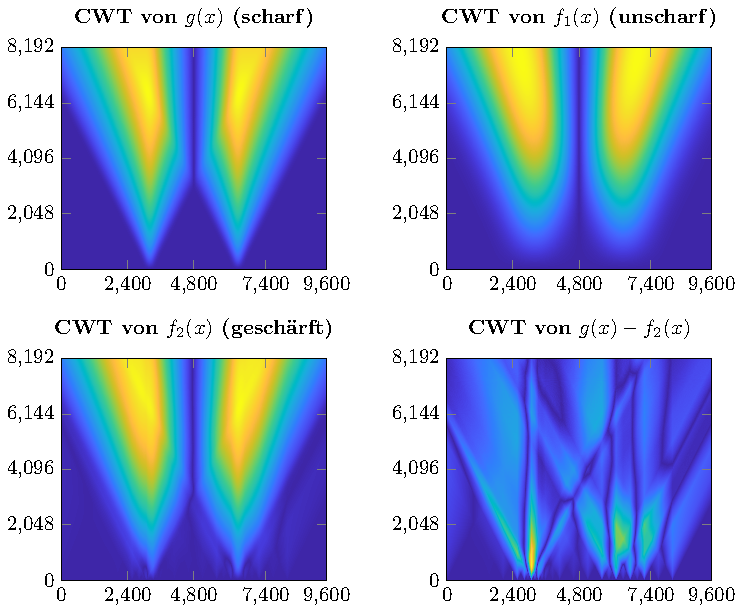
\includegraphics[width=0.9\textwidth]{./papers/deconvolve/pictures/cwt.pdf}
\caption{stetige Transformationen\label{deconvolve:cwt}}
\end{figure}


\section{Bild}
\rhead{Bild}
Dieser Teilerfolg soll nun auch auf zwei Dimensionen, also ein Bild angewendet werden.
Dafür wird ein etwas verschwommenes Dreieck, wie abgebildet links in \ref{deconvolve:example}, als Versuch verwendet.
Die Grösse des Bildes beträgt 9600x9600 Pixel, analog den 9600 Samples der obigen Funktion.
Vorteil diese Bildes ist es, dass es Zeilen- und Spaltenweise genau gleich wie das 1D-Signal behandelt werden kann.
\begin{figure}[h]
\centering
\includegraphics[width=0.9\textwidth]{./papers/deconvolve/pictures/dreieck.pdf}
\caption{Beispielbild\label{deconvolve:example}}
\end{figure}

Die Parameter $m$ und $\alpha$, die vorher für jedes Level bestimmt wurden, bleiben erhalten.
Die Funktion aus \eqref{deconvolve:funktion} wird also auf alle Level gleich wie oben ausgeführt.
Dies geschieht einmal Zeilen- und Spaltenweise.
Insgesamt wird also 19200 mal eine Analyse mit der dikreten Wavelet-Transformation gemacht.
Danach wird das arithmetische Mittel der beiden korrigierten Bilder genommen:
$$f_\text{sharp}(x,y)=\frac{f_\text{rows}(x,y)+f_\text{cols}(x,y)}{2}.$$
$f_\text{sharp}$ bezeichnet hierbei das Endergebnis, $f_\text{rows}(x,y)$ und $f_\text{cols}(x,y)$ sind die Zeilen-, bzw. die Spaltenweise \glqq geschärften\grqq{} Varianten des ursprünglichen Bildes.
Abbildung \ref{deconvolve:ergebnis} zeigt das daraus resultierende Ergebnis.
\begin{figure}[h]
\centering
\includegraphics[width=0.7\textwidth]{./papers/deconvolve/pictures/dreieck_sharp.png}
\caption{Ergebnis\label{deconvolve:ergebnis}}
\end{figure}
 
Eine Verbesserung ist nicht zu erkennen. Wo vorher der Rand verschwommen war, sind jetzt einfach starke Schwingungen aufgetreten.

\section{Schlussfolgerung}
\rhead{Schlussfolgerung}
Innerhalb dieser Seminararbeit konnte keine fertige Funktion zur Bildschärfung erarbeitet werden.
Der bestehende Ansatz mit der Beziehung \eqref{deconvolve:funktion}, welche zwei Freiheitsgrade beinhaltet, könnte aber noch verfeinert werden.
Die beiden Parameter $m$ und $\alpha$ wurden hier mithilfe einer eindimensionalen Funktion $g(x)$ (Abbildung \ref{deconvolve:1d}) festgelegt.
Es wäre daher vielleicht möglich, durch geschickteres wählen dieser Parameter auf ein besseres Ergebnis zu kommen.
Ausserdem ist die Anwendung auf das Bild noch nicht ausgereift.
Es wurden auch nur das Haar- bzw. db1-Wavelet verwendet.
Ein ähnliches Vorgehen, z.B. mit höheren Debauchies-Wavelets wäre sicher ein Versuch Wert.

Folgende Punkte scheinen aber die Hauptgründe zu sein, den bestehenden Ansatz zu verwerfen:
\begin{itemize}
	\item Es stellte sich als problematisch heraus, die Koeffizienten auf den einzelnen Level zu verändern, bzw jede Zeile in Abbildung \ref{deconvolve:y1_cwt} unabhängig von den anderen zu verstärken oder abzuschwächen.
	
	Die Wavelet-Transformation hat ja zwei Dimensionen (Dilatation $a$ und Translation $b$) und somit muss \glqq Masse \grqq{} in der Ebene, also zwischen Level und nicht nur auf einer Zeile nach links oder rechts verschoben werden.
	Ändert man auf einem Level etwas, so muss die Auswirkung auf die anderen Level unbedingt berücksichtigt werden.
	\item Wie beim eindimensionalen Versuch beobachtet, darf nicht davon ausgegangen werden, dass eine lokale Änderung auf einem Level nur diese Stelle beeinflusst.
	Folglich könnte sich eine Manipulation an einem anderen Ort, der sich weiter weg von der zu schärfenden Stelle befindet, umgekehrt eben auf diese Stelle auswirken. 
\end{itemize}

Diese zwei Erkenntnisse sollte man immer im Hinterkopf behalten, wenn man die Wavelet-Transformation vergleichbar einsetzten will.





\printbibliography[heading=subbibliography]
\end{refsection}
